\section{Introduction}
In this chapter we build on the empirical heat maps of Chapter 2. First, we develop a statistical model for spatial variation in hitter success probabilities. This involves generalized linear models (GLMs) with biomechanical covariates. Second, we focus on heat map confidence intervals, by taking a look at current best practices, and providing an alternative. The final section presents a vignette for our newly launched R package {\bf mapapp}, which automates creating interactive heat map confidence intervals using the R package {\bf shiny} \citep{Shiny}.

\section{A Generalized Linear Model for Hitter Success Probabilities} % =========================

\subsection{Preliminaries}

We aim to create an interpretable statistical model to explain spatial variation of success probabilities through the hitting zone. Nonparametric methods, lacking contextual parameters, limit interpretability, and we therefore use a parametric approach that involves biomechanically interpretable covariates. Existing research analyzes the biomechanics of the baseball swing \citep{Welch1995}, but no research links those results to actual spatial hitting results in a statistical model. 

As we move into describing and writing out a statistical model to relate swing success to batter biomechanics, the simple notation from Chapter 2 does not suffice. Strictly speaking, the data contain a compound nesting structure:

\begin{enumerate}

\item a swing occurs within an at-bat;

\item an at-bat occurs with a batter and a pitcher;

\item an at-bat occurs within a game;

\item a game occurs within a season.

\end{enumerate}

Given this structure, we let $Y_{ijk\ell mn}$ denote the Bernoulli outcome on swing $i$ for at-bat $j$ against pitcher $k$ for batter $\ell$ in game $m$ during season $n$. Here,

\begin{itemize}

\item $i = 1,\ldots,I_{jk\ell mn}$, where $I_{jk\ell mn}$ is the number of swings during at-bat $j$ against pitcher $k$ for batter $\ell$ in game $m$ of season $n$.

\item $j = 1,\ldots,J_{k\ell mn}$, where $J_{k\ell mn}$ is the number of at-bats against pitcher $k$ for batter $\ell$ in game $m$ of season $n$.

\item $k = 1,\ldots,K_{\ell mn}$, where $K_{\ell mn}$ is the number of pitchers that face batter $\ell$ in game $m$ of season $n$.

\item $\ell = 1,\ldots,L_{mn}$, where $L_{mn}$ is the number of batters in game $m$ of season $n$.

\item $m = 1,\ldots,M_n$, where $M_n$ is the number of games in season $n$.

\item $n = 1,\ldots,10$, representing the seasons 2007 through 2016.

\end{itemize}

Also available in the data, associated with each swing, is the location of the pitch in the two-dimensional vertical face of the hitting zone. We let $\mathbf{s}_{ijk\ell mn} = (x_{ijk\ell mn},y_{ijk\ell mn})$ denote this two-dimensional pitch location. The origin, $\mathbf{s} = (0,0)$, lies at the midpoint of the front edge of home plate at ground level. From the home plate umpire's vantage point, pitches to the left of the origin correspond to negative values of $x_{ijk\ell mn}$. Pitches that bounce before reaching home plate correspond to negative values of $y_{ijk\ell mn}$.

Since our interest lies in modeling swing success with respect to a batter's biomechanics and pitch location, we make the simplifying assumptions that that relationship remains unchanged from at-bat to at-bat, from pitcher to pitcher, from game to game and from season to season.\footnote{See Section \ref{EHZHM} for a brief discussion of this assumption.} This leaves us with simplified notation, with $Y_{ij}$ now denoting the Bernoulli outcome of the $i^{th}$ swing for the $j^{th}$ batter. To be clear, the indices are now:

\begin{itemize}

\item $i  = 1,\ldots,N_j$, where $N_j$ denotes the total number of swings that batter $j$ takes over all at bats, against all pitchers, in all games, during all seasons.

\item $j = 1,\ldots,N$, where $N$ is the total number of batters in the dataset, in this case $N = 1,932$\footnote{Right-handed hitters.}.

\end{itemize}

Similarly, we simplify the notation for pitch location to $\mathbf{s}_{ij} = (x_{ij},y_{ij})$ using the same indices just itemized.

In this chapter, we consider biomechanical covariate information, $\mathbf{X}_{ij}(\mathbf{s}_{ij})$, that depends upon the location of the pitch, and we take:
\bdm
Y_{ij}|\mathbf{X}_{ij}(\mathbf{s}_{ij}) \stackrel{ind}{\sim} \mbox{Bernoulli}(\pi_{ij})
\edm
with
\bdm
\log\left(\frac{\pi_{ij}}{1-\pi_{ij}}\right) = \mathbf{X}_{ij}(\mathbf{s}_{ij})\beta,
\edm
where $\beta$ are unknown regression parameters.\footnote{We extend this model to include a spatial random effect in Chatper 4.}  We describe the biomechanical covariates next.

\subsection{Rotational Biomechanics} % ==============

Why does Jhonny Peralta, and why do hitters in general, hit pitches in some locations better than others? We propose that biomechanics underpin hitting spatial swing success probabilities. Given a choice, athletes in other sports carefully position their ball before swinging. Consider golf, a sport with a stationary ball, where the athlete chooses the exact athlete-to-ball distance, depth, and angle. 
  \begin{figure}[H]
	\centering	
	\includegraphics[scale=.45]{Images/Golf.jpg}
  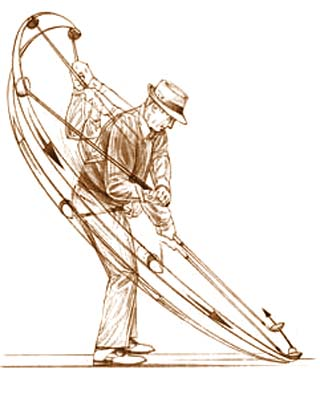
\includegraphics[scale=.6]{Images/Snead.jpg}
	\caption{Golfers position themselves with careful precision in relation to the ball, to achieve optimal impact. Deviations from this ideal lead to biomechanical adjustments and suboptimal results \citep{Cochran2005}.}
	\label{fig:golf}
	\end{figure}
Indeed, golfers position themselves very precisely in relation to the ball to achieve optimal impact \citep{Cochran2005}. If the impact point deviates from the optimal location, biomechanical adjustments hurt performance. Or consider tennis, similar to baseball in that a moving ball approaches, but different in that the player has greater freedom to position him/herself relative to the incoming ball. Once again, tennis players strive to hit the ball at a specific point in their stroke, a precise distance from the ground and from their body, with precise depth \citep{Elliott2006}. 
  \begin{figure}[H]
	\centering	
	\includegraphics[scale=.4]{Images/tennis2.jpeg}
	\caption{Tennis players strive to hit the incoming tennis ball at a precise height and distance from their torso. Deviations from this ideal height and distance lead to a series of biomechanical adjustments, and ultimately suboptimal results \citep{Elliott2006}.}
	\end{figure}
As with golf, if the point of impact deviates from from the optimal location, biomechanical adjustment ensue, and performance suffers. Tennis provides a strong example, because players have {\it some} control over the point of impact, and results demonstrate the consequence of varying points of impact. For example, even novice viewers observe that a player barely reaching a ball returns it, on average, with less velocity and precision than a ball he/she has time to set up for.  

We believe the same dynamics affect baseball hitting. In baseball, however, the hitter must react to an unpredictable ball location, without the ability to reposition himself in response to the location and trajectory of the incoming pitch.

\subsection{Biomechanical Covariates}

For now we focus on biomechanical information content captured in pitch locations, though technical advancements may at some point allow others to also incorporate batter-specific physical characteristics. To obtain biomechanical covariates with respect to pitch location, we convert rectangular coordinate pitch locations to polar coordinates with a translated origin. With the proper origin translation, this switch infuses pitch locations with hitter-to-ball relationship information. Based on a conversation with Glen Fleisig of the American Sports Medical Institute, we locate the polar origin at the bat's approximate in-swing moment-of-inertia \citep{Fleisig}. In Figure \ref{fig:polar} we illustrate this origin shift to the bat's approximate MOI, for a league average 6'2" hitter. The MOI coincides approximately with the intersection of the bat line at the moment of contact and the hitter's axis of rotation \citep{Welch1995}.
  \begin{figure}[H]
	\centering
	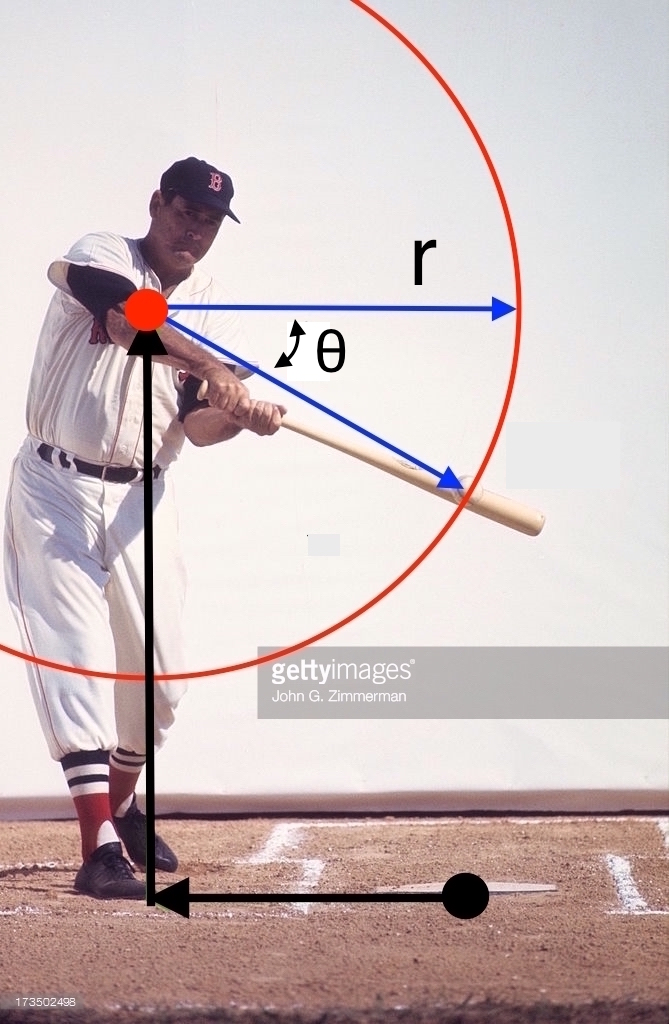
\includegraphics[scale=.16]{Images/WilliamsPolar.jpg}
	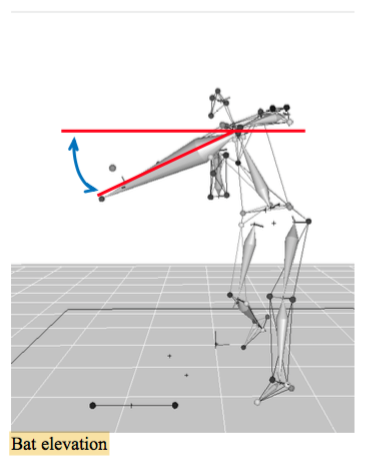
\includegraphics[scale=.07]{Images/Elevation.jpg}
	\caption{Ted Williams in ``The Science of Hitting,'' and baseball swing kinematic analysis at the American Sports Medical Institute \citep{Fortenbaugh2011}. We translate the origin (black dot) and rectangular coordinates to the new origin (red dot) in polar coordinates. We located the new origin at the bat's approximate moment of inertia (MOI) \citep{Fleisig}. Polar coordinates component $r$ gives the MOI-to-ball distance, and $\protect\theta$ gives the bat ``elevation.''}
	\label{fig:polar}
	\end{figure}
Polar coordinate $r$ measures the distance, at contact, from the bat's MOI to the ball; and polar coordinate component $\theta$ measures bat {\it elevation}, or the angle below horizontal of the bat line, as shown in the kinematic analysis image on the right \citep{Fortenbaugh2011}. 

As in golf and tennis, hitter-to-ball distances---too close to/far from the hitter, above/below the ideal point of impact---affect hitting performance. We use $r_{ij}$ and $\theta_{ij}$ terms for $\pmb{X}_{ij}(\pmb{s}_{ij})$ in equation 3.1.

\subsection{Generalized Linear Model} % =========================

Further biomechanical research extends beyond the scope of this study. Therefore, without biomechanical knowledge to inform us otherwise, we use $r$ and $\theta$ linear, quadratic, and interaction terms as covariates in our GLM linear predictor; $\pmb{X}_{ij}(\pmb{s}_{ij}) = \{r_{ij}, \theta_{ij}, r_{ij}\theta_{ij}, r_{ij}^{2}, \theta_{ij}^{2}, r_{ij}^{2}\theta_{ij}^{2}\}$. With $6 \times 1$ covariate vector $\pmb{X}_{ij}(\pmb{s}_{ij})$ in hand, we can define $\pmb{\beta}_{j}' =  \{\beta_{j0}, \beta_{j1}, \dots, \beta_{j6}\}$, and recall:

\begin{equation} \label{eq:glm}
\text{logit}(p_{ij}|\pmb{X}_{ij}(\pmb{s}_{ij})) = \pmb{X}_{ij}(\pmb{s}_{ij}) \pmb{\beta}_{j}.
\end{equation}

Note that given a hitter $j$, and pitch location $\pmb{s}_{ij}$, the elements of $\pmb{X}_{ij}$ are simply a trigonometric function of $\pmb{s}_{ij}$ and the translated origin.

As a first step in exploring the effectiveness of the approach developed above, we fit the model to Johnny Peralta's data (see Chapter 2). Let $j = P$, denoting player (P)eralta. We use Peralta's $n_{\text{P}} = 9177$ observed swings, and fit the model using the R \verb|glm()| function , finding maximum likelihood estimates of $\pmb{\beta}_{\text{P}}$ with the iteratively reweighted least squares algorithm (IRLS) \citep{Myers2012}. In Figure \ref{fig:empvsfit} we show the Peralta empirical and fitted heat maps.
  \begin{figure}[!ht]
    \centering
    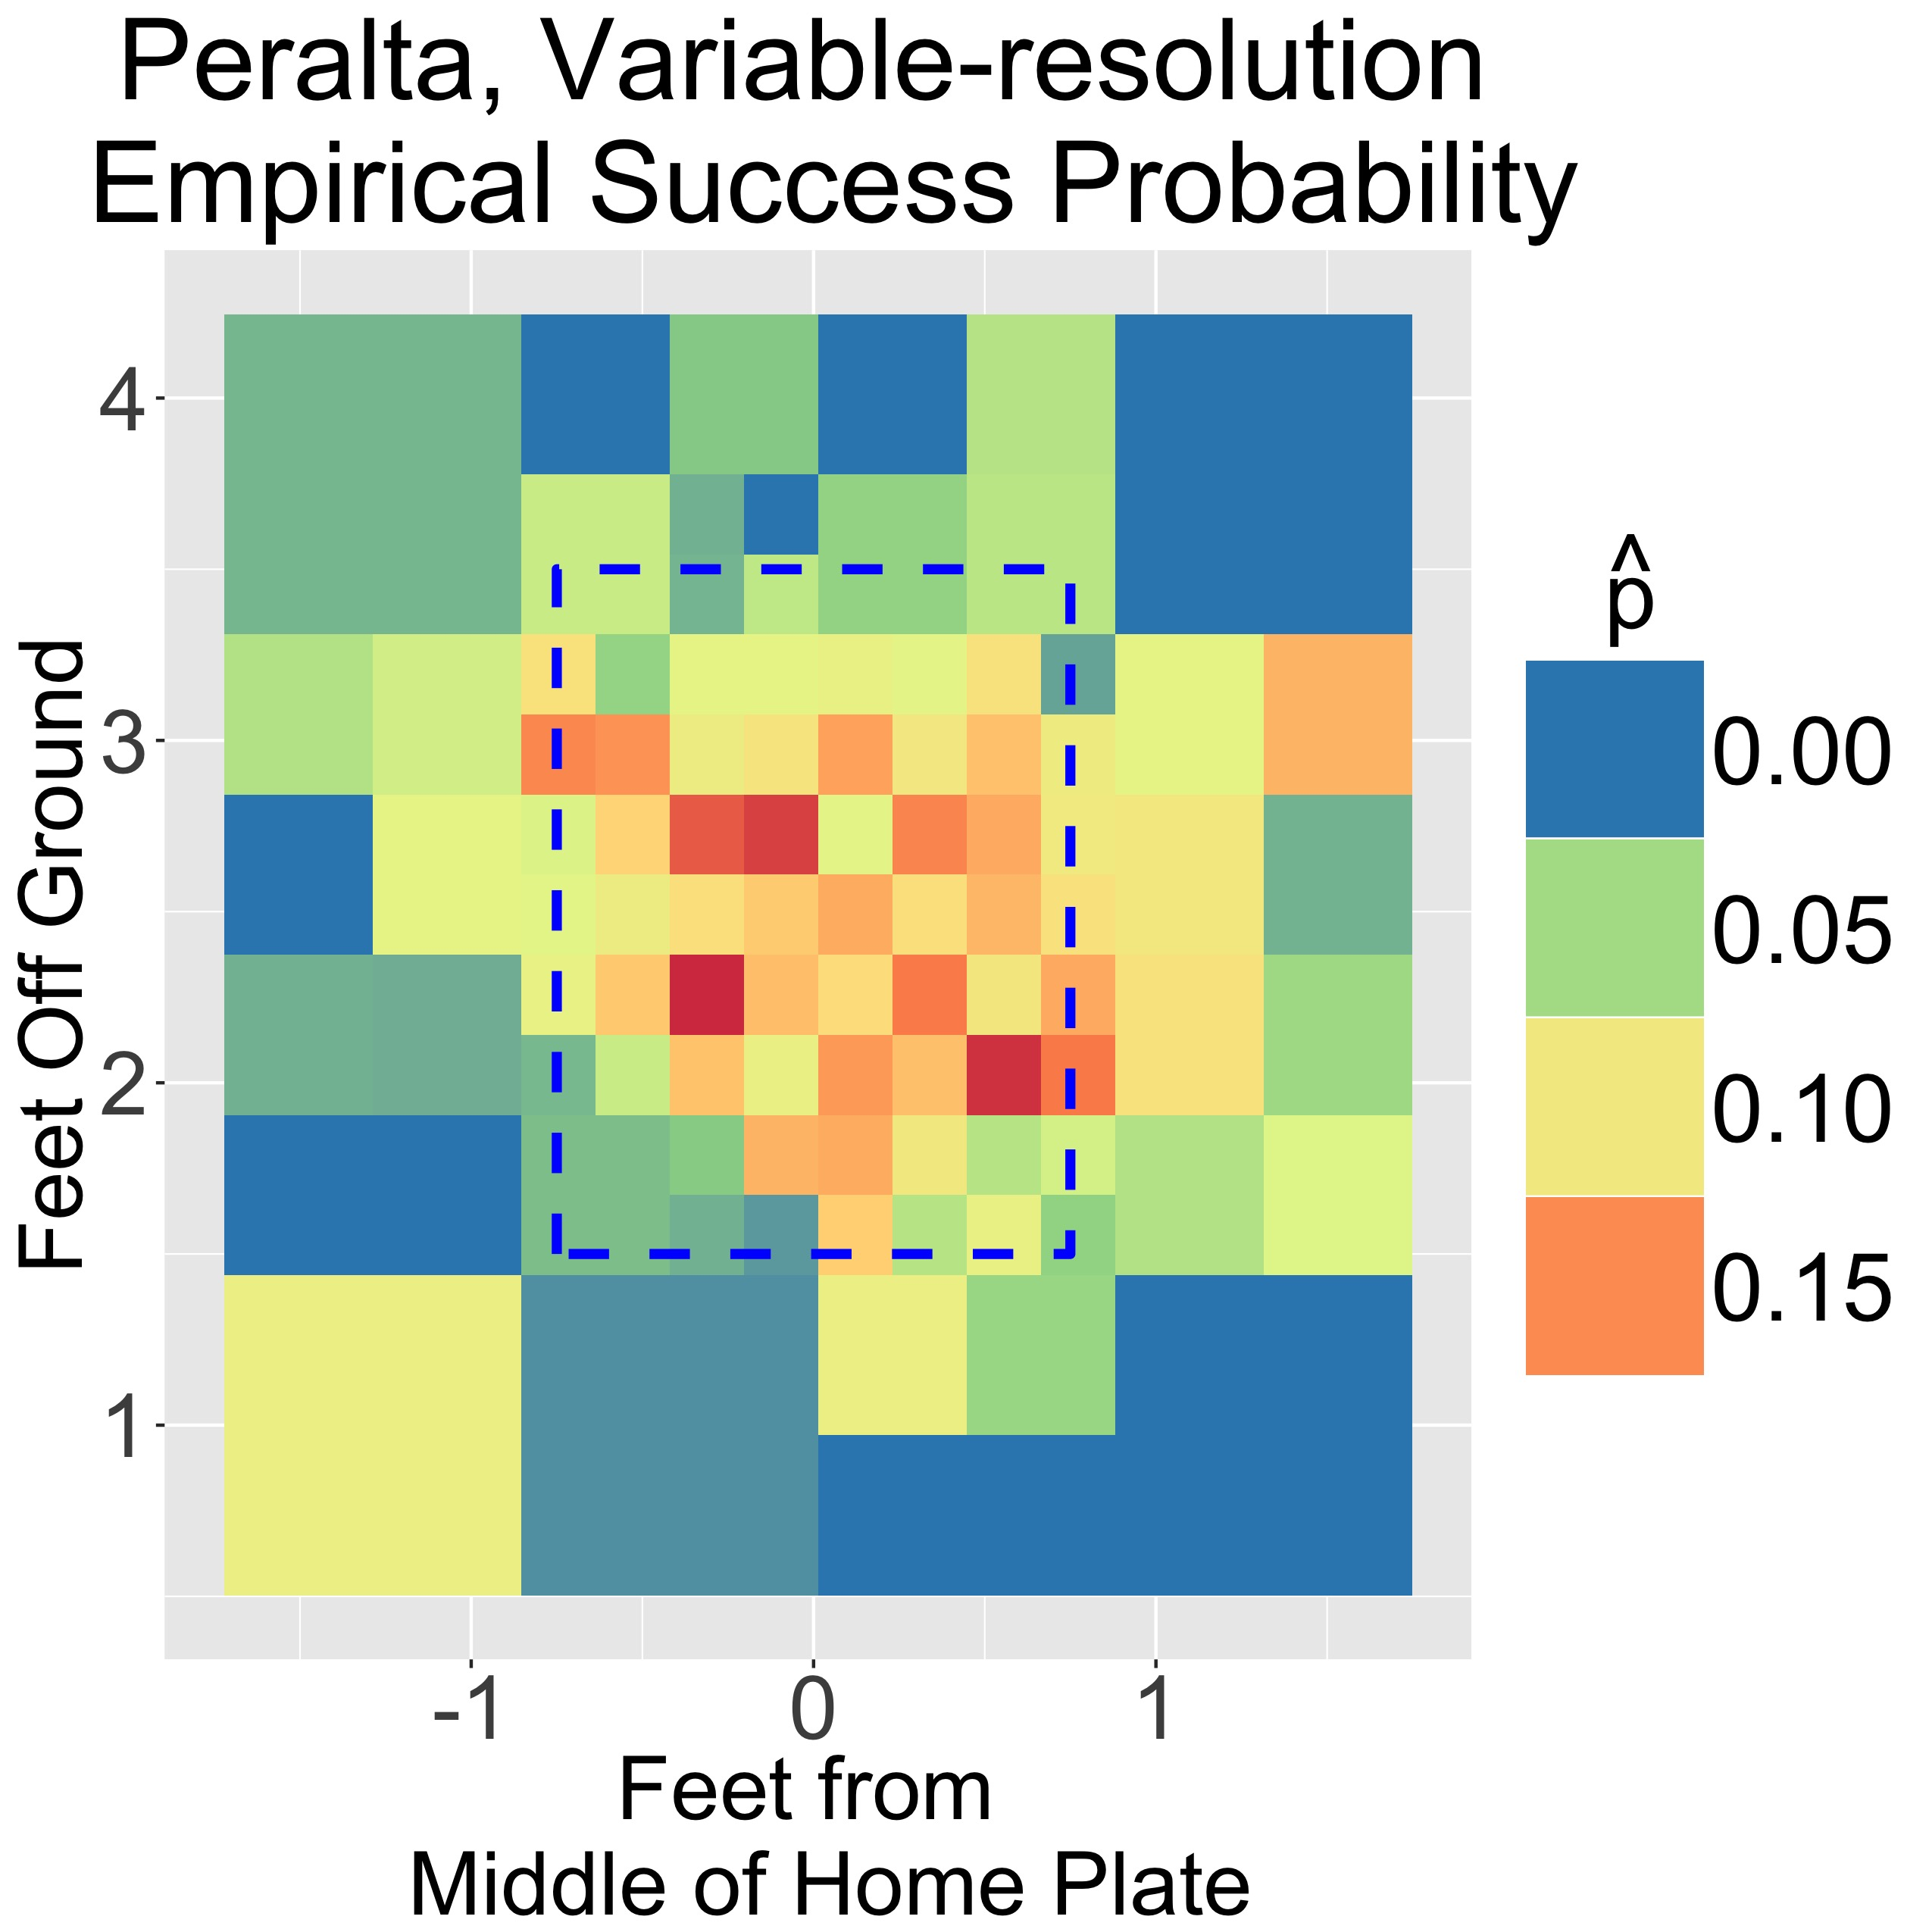
\includegraphics[scale=.08]{Images/Peralta_var-res.jpg}
    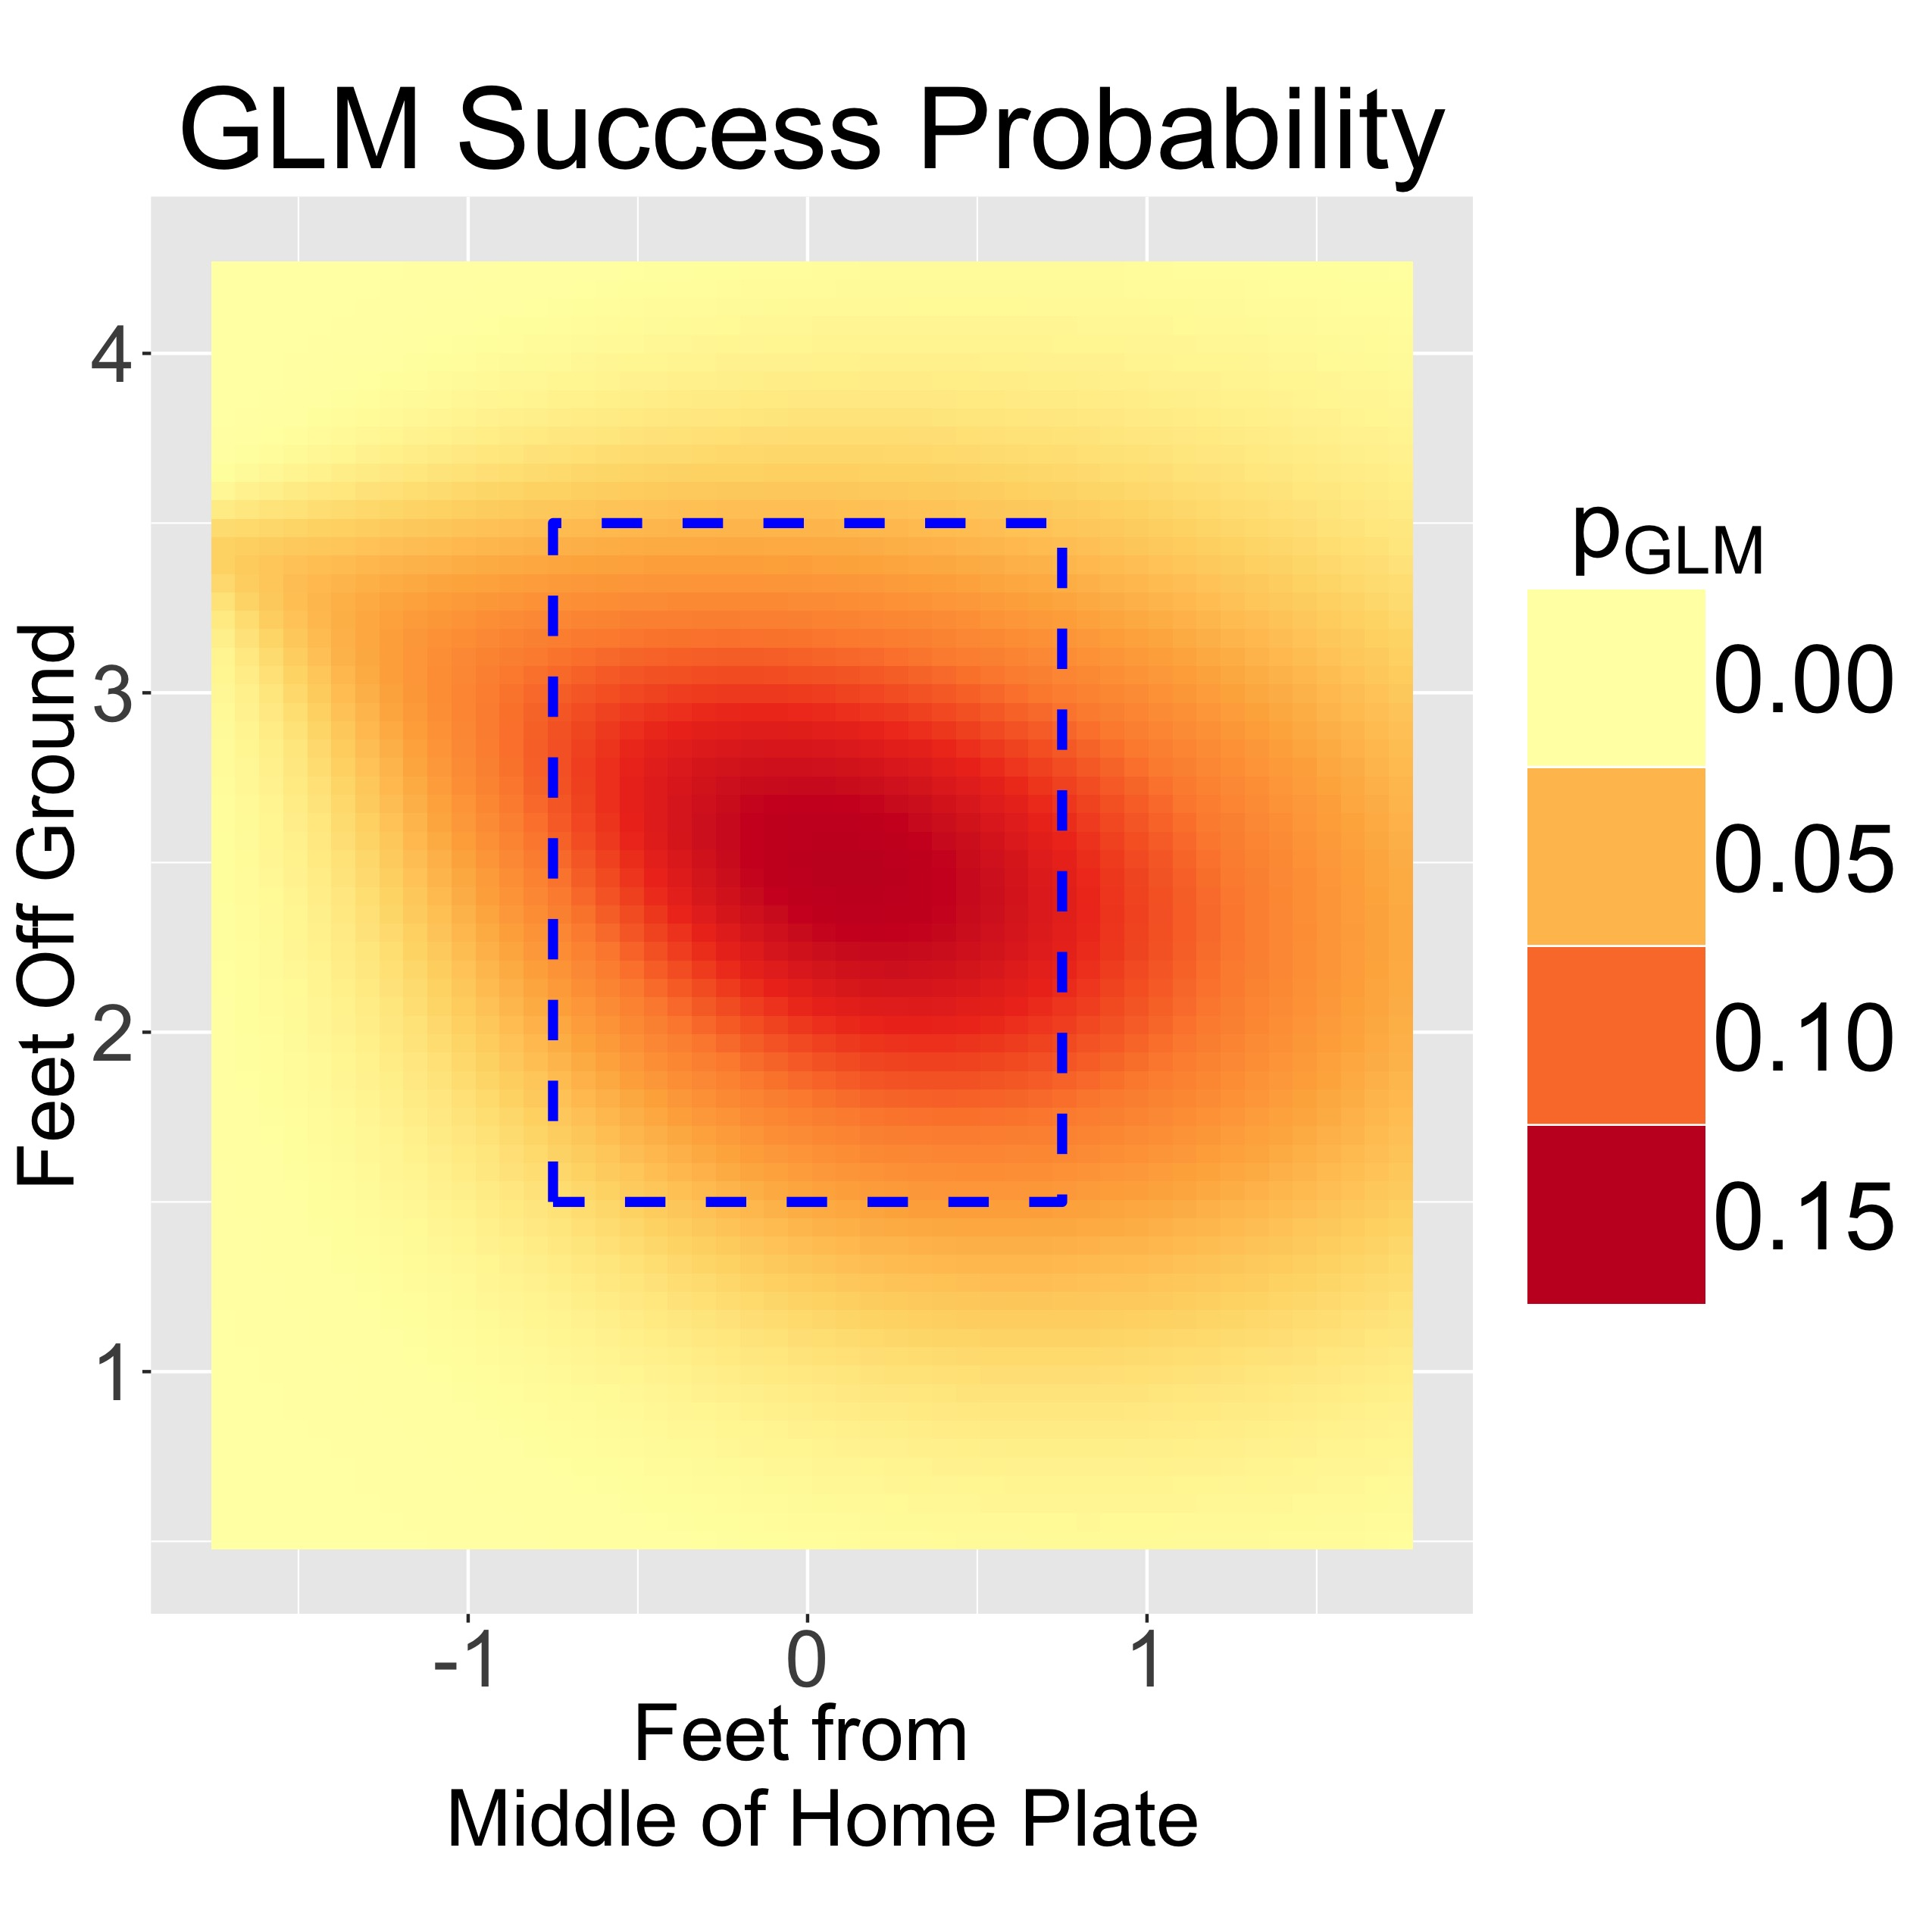
\includegraphics[scale=.08]{Images/Peralta_fit.jpg}
    \caption{Jhonny Peralta variable-resolution heat map and generalized linear model fit. The general shapes of higher success probability regions seem to match. Both maps show lower success probabilities near the borders of the hitting zone, especially those borders further from the center of the water drop shape.}
    \label{fig:empvsfit}
  \end{figure}
We turn to an established goodness of fit test for statistical validation.

\subsection{Hosmer-Lemeshow Goodness of Fit Test} % ================

The widely used Pearson $\chi^{2}$ test assesses goodness of fit for models with covariates that provide natural groupings \citep{Pagano2000}. Continuous covariate models, however, need an imposed grouping mechanism for a similar test. The Homer-Lemeshow test uses a grouping mechanism to imitate Pearson $\chi^{2}$ test structure, and tests logistic regression model goodness of fit \citep{Hosmer2013}. Conceptually, the test compares the observed results in each grouping to the expected results under the null hypothesis of a well fit model, and then assesses the overall degree to which observed and expected results differ. Under the null hypothesis the difference approximately follows a $\chi^{2}$ distribution. 

To construct the Hosmer-Lemeshow test, first define Bernoulli outcome vector $\pmb{y} = \{y_{1}, y_{2}, \dots, y_{n}\}^{\text{T}}$, and logistic regression model fitted probability vector $\hat{\pmb{y}} = \{\hat{p}_{1}, \hat{p}_{2}, \dots, \hat{p}_{n}\}^{\text{T}}$, where $E(y_{i}) = p_{i}$. Next, arrange fitted values $\hat{p}_{1}, \hat{p}_{2}, \dots, \hat{p}_{n}$ in ascending order, and divide them into $g$ evenly spaced groups, partitioned by the quantiles: $\frac{1}{g}, \frac{2}{g}, \dots \frac{g}{g}$. For example, $\text{Group 1} = \{\hat{p}_{i}\text{ }|\text{ }0 < \hat{p}_{i} < p_{1}\}$ where $\hat{\text{F}}_{\hat{p}}(p_{1})=1/\text{g}$, for the empirical cumulative distribution function $\hat{\text{F}}_{\hat{p}}(p)$. 

To define the Hosmer-Lemeshow goodness of fit test statistic, let $n_{k}$ be the number of observations in quantile group $k$, for $k = 1, \dots, g$. Then,
$$ \widehat{C} = \sum_{k=1}^{g} \left[ \frac{(\text{o}_{1k}-\hat{e}_{1k})^{2}}{\hat{e}_{1k}} + \frac{(\text{o}_{0k}-\hat{e}_{0k})^{2}}{\hat{e}_{0k}}  \right], $$
where
$$ \text{o}_{1k} =  \sum_{j=1}^{n_{k}}y_{j},$$
$$ \text{o}_{0k} =  \sum_{j=1}^{n_{k}}(1-y_{j}),$$
$$ \hat{e}_{1k} = \sum_{j=1}^{n_{k}}\hat{p}_{j}, \text{ and }$$
$$ \hat{e}_{0k} = \sum_{j=1}^{n_{k}}(1-\hat{p}_{j}).$$
Simplifying, 
$$ \widehat{C} = \sum_{k=1}^{g} \frac{(\text{o}_{1k}-n_{k}\bar{\hat{p}}_{k})^{2}}{n_{k}\bar{\hat{p}}_{k}(1-\bar{\hat{p}}_{k})},$$
where $\bar{\hat{p}}_{k}$ equals the average of the group k predicted probabilities:
$$\bar{\hat{p}}_{k} = \frac{1}{n_{k}}\sum_{j=1}^{n_{k}}\hat{p}_{j}.$$
Notice $\widehat{C}$ matches the Pearson $\chi^{2}$ statistic under this grouping structure. Here, $\widehat{C}$ follows, approximately, a chi-sq distribution with g-2 degrees of freedom \citep{Hosmer1980}, for the standard goodness-of-fit null and alternative hypothesis.
\begin{align}
H_{0}: & \text{ Model well fit.} \\
H_{1}: & \text{ Model not well fit.}
\end{align}
We use g = 10, following the \cite{Hosmer2013} recommendation based on their simulations \citep{Hosmer1980}. The test statistic for Jhonny Peralta's data, $\widehat{C} = 4.3758$, with eight degrees of freedom, gives a p-value of p = 0.8217. This lends credibility to the biomechanical covariate approach. This validation will suffice for now, and it sets the stage for the more substantial innovation in this chapter, an interactive heat map confidence interval.

\section{Interactive Heat Map Confidence Intervals}

\subsection{Motivation}

A heat map presents a two dimensional surface of point estimates. Each (x,y) point on the surface maps a point estimate of a parameter to a color. As discussed in Chapter 2 with empirical heat maps, heat maps of model estimates also efficiently communicate the behavior of the parameter point estimates across a spatial domain. Often the usefulness of a point estimate, however, depends on some measure of the variability of that estimate, and therein lies the challenge: How do we effectively present confidence intervals for heat maps? This problem exists in numerous areas of application---in fact, any field where heat maps are used \citep{Emerson}. 

\subsection{Current Best Practices}

Current heat map confidence interval technology consists of including two additional heat maps along with the point estimate map: a lower bound heat map and an upper bound heat map. Sometimes the presentation includes maps for additional percentiles. For example, \cite{Cross2015} provide the following collection of heat maps to communicate prediction variability.
  \begin{figure}[H]
	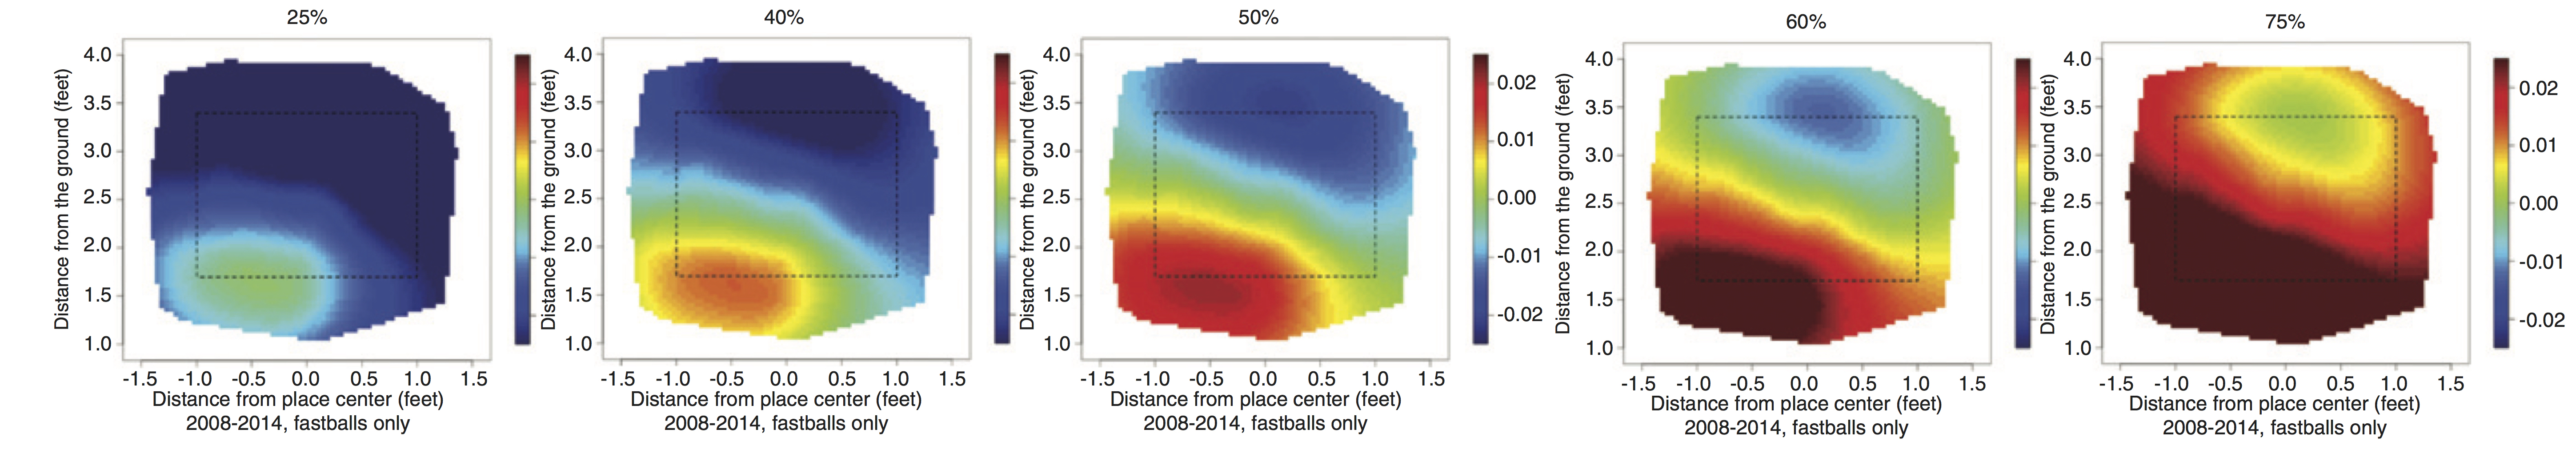
\includegraphics[scale=.07]{Images/CrossHMCI.jpg}
	\caption{In line with best practices, \cite{Cross2015} present four percentiles to convey confidence interval information for the point estimate heat map in the center. Plots reproduced from cite{Cross2015}, Figure 8}
	\end{figure}
We find this heat map confidence interval method to be relatively inaccessible, both conceptually and intuitively, especially compared to typical confidence interval for a univariate parameter. For example, consider a hypothetical parameter, $\theta$, with point estimate $\hat{\theta} = 2$, and hypothetical confidence interval for $\theta$ of (0,4). This combination makes plain its information content and structure; our familiarity with the number line contributes to easy comprehension.
  \begin{figure}[H]
  \centering
	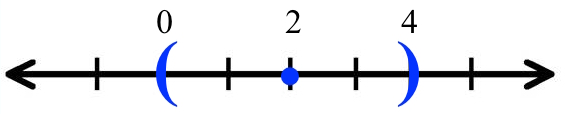
\includegraphics[scale=.6]{Images/NumberLine.jpg}
	\caption{A confidence interval on the number line. Our brain readily understands ``(0, 4),'' and interprets it as a segment of the familiar number line. } % A heat map CI, on the other hand, exists on the color spectrum; our brain does not so easily understand and fill in missing intervals of the color spectrum.
	\end{figure}
While one quickly, intuitively, and easily understands the content of the number line, we typically cannot so easily fill in missing segments of the color spectrum. With heat map confidence intervals, {\it colors} represent the point estimate and confidence bounds. A point estimate of ``green'' with a confidence interval of (purple, red) is simple but not straightforward to interpret or understand. In Figure \ref{fig:colorCI}, for example, we show lower and upper color bounds to represent a confidence interval, but without a quantitative x-axis, it is difficult to really know what this means.
  \begin{figure}[H]
  \centering
	
\includegraphics[scale=.75]{Images/Lower.jpeg}
	
\includegraphics[scale=.75]{Images/SpectrumPE.jpg}
	
\includegraphics[scale=.75]{Images/Upper.jpeg}
	\caption{This representation of a confidence interval on the color spectrum demonstrates the interpretive challenge. What stream of colors exist between each bound and the point estimate?}
	\label{fig:colorCI}
	\end{figure}
We might understand a color confidence interval more easily if we include the entire interval as in Figure \ref{fig:specint}.
  \begin{figure}[H]
  \centering
	
\includegraphics[scale=.65]{Images/SpectrumCI.jpg}
	\caption{We understand a colored confidence interval without missing color segments, with the entire color confidence interval visible}
	\label{fig:specint}
	\end{figure}
This presentation seems to improve comprehension. But, how do we achieve this for a heat map {\it surface}? A continuous model maps uncountably many point estimates on a surface, to a color, and this makes producing a visible color spectrum confidence interval for each point estimate unfeasible. We propose a dynamic, interactive solution implemented with RStudio's Shiny and package {\bf shiny} \citep{Shiny}, \citep{RStudio}.

\subsection{Shiny Implementation}
The inimitable RStudio created the Shiny framework to facilitate interactive web application development. Deployed directly out of the RStudio integrated development environment (IDE) \citep{IDE} or on the web, Shiny applications provide a powerful new tool for presenting analytic results. Ordinarily one needs to program in HTML to present results on interactive webpages, but Shiny provides a platform to enable such development directly from R. We developed a heat map confidence interval method and used Shiny to implement it.

Recall the GLM model heat map for Johnny Peralta's data. In Figure \ref{fig:LPU} we show lower and upper pointwise 95\% confidence interval heat maps, calculated with the variance-covariance estimates from the IRLS procedure \citep{Myers2012}.
  \begin{figure}[H]
	\centering
	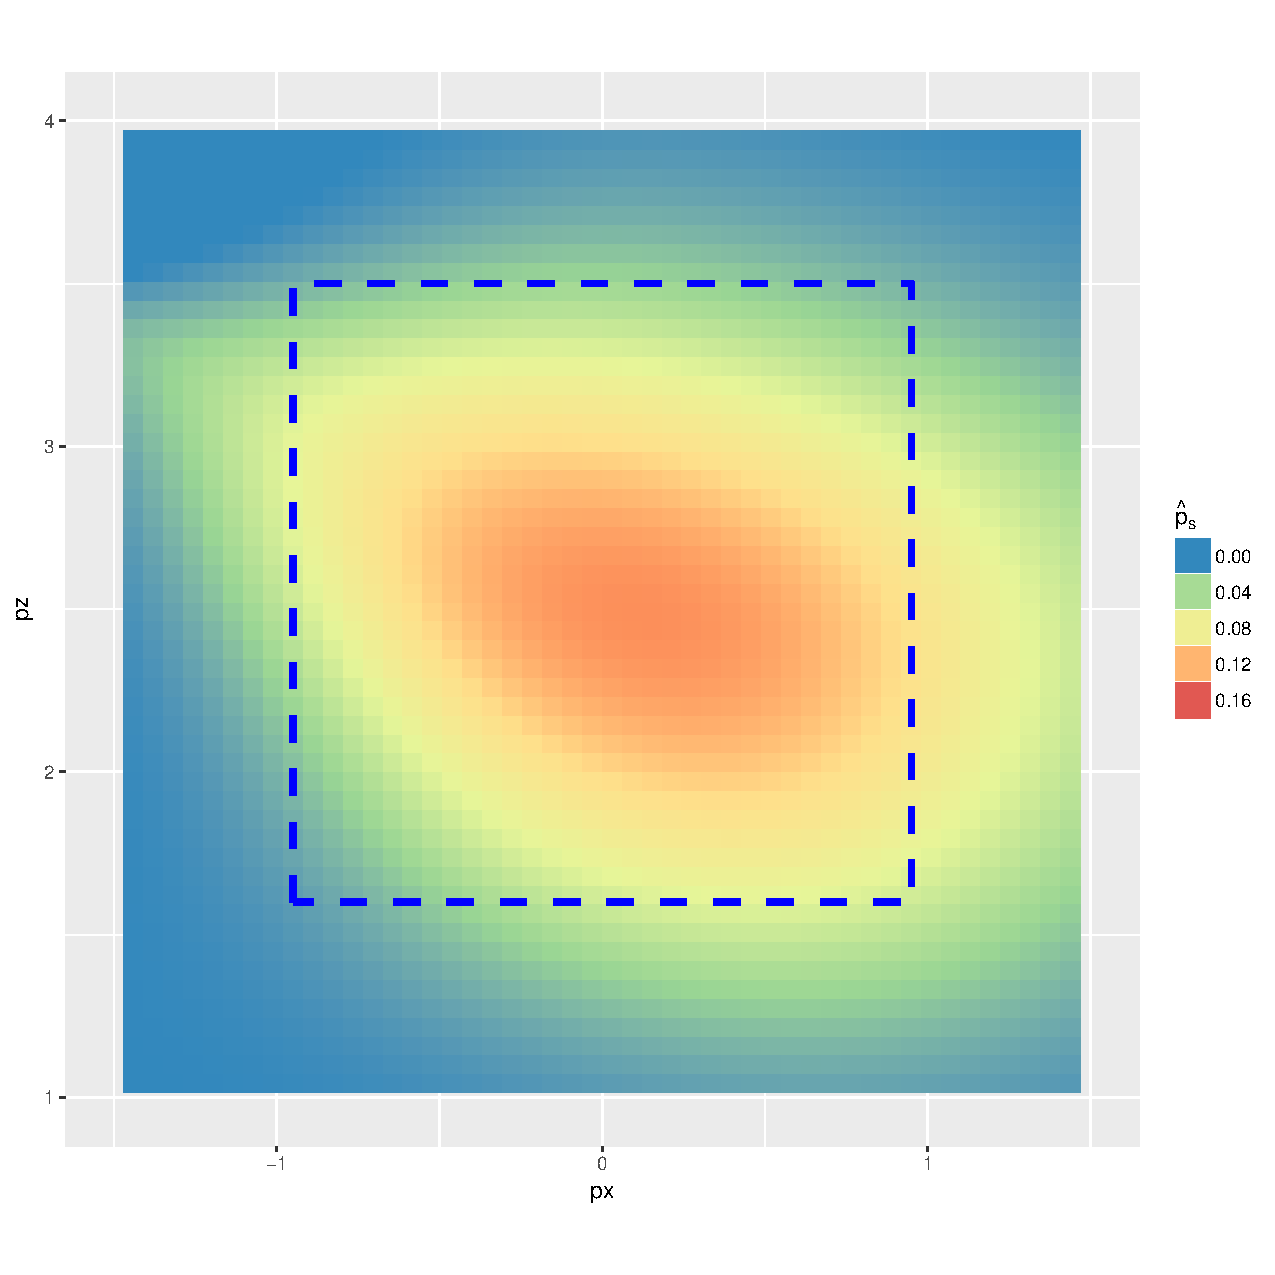
\includegraphics[scale=.2]{Images/Lower.pdf}
	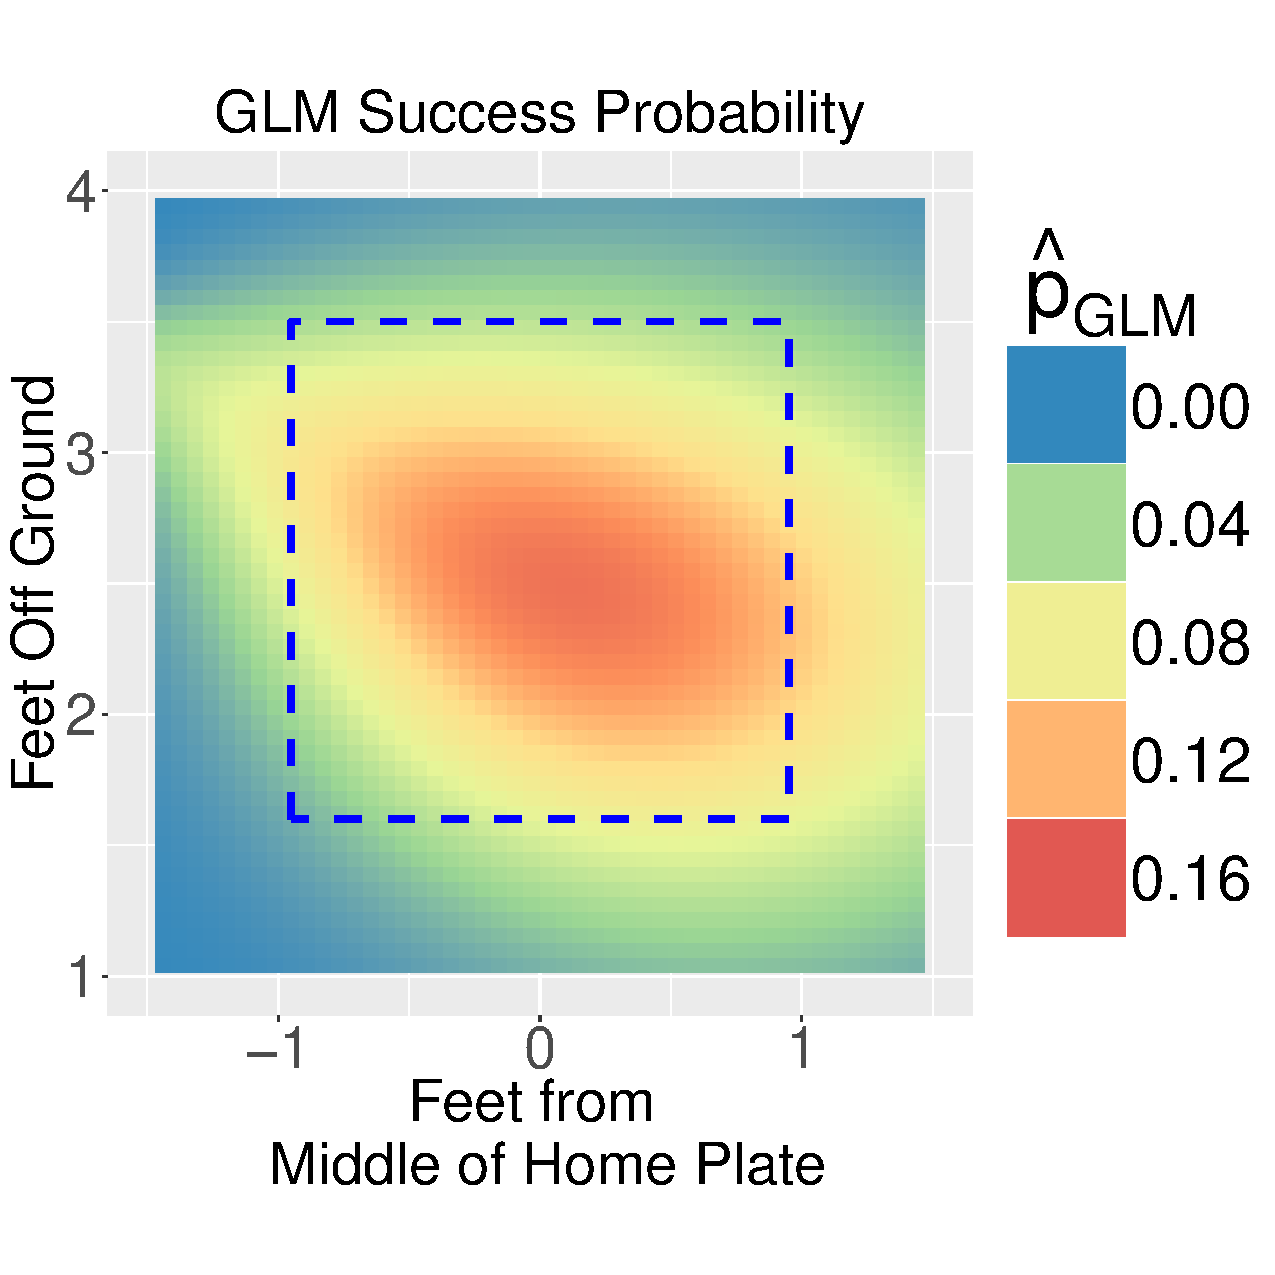
\includegraphics[scale=.25]{Images/Perralta_fit.pdf}
	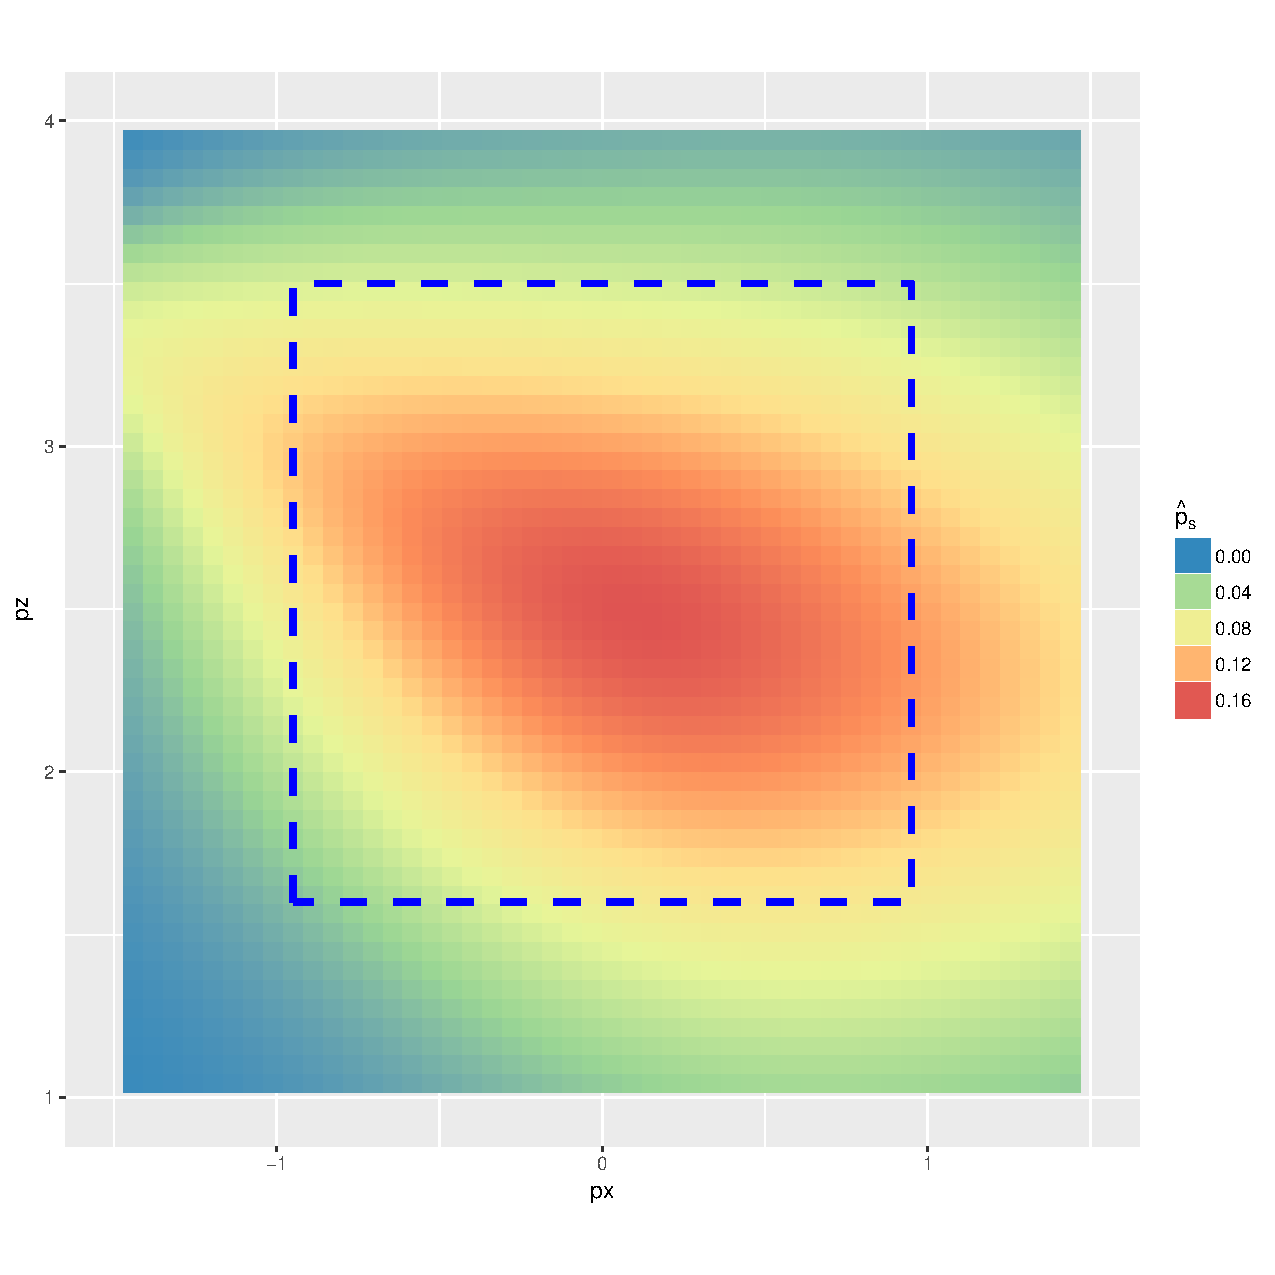
\includegraphics[scale=.2]{Images/Upper.pdf}
	\caption{Current best practices for a heat map confidence interval. The generalized linear model fit for Jhony Peralta in the center, the pointwise 95\% confidence interval lower/upper bounds on the left/right. Our interactive, dynamic heat map confidence intervals ease understanding.}
	\label{fig:LPU}
	\end{figure}
The heat map on the left gives the lower bound of the 95\% confidence interval, the heat map in the middle gives the model fit point estimates, and the heat map on the right gives the upper bound of the 95\% confidence interval. We removed labels from the left and right heat maps to de-clutter the figure. The data visualization challenge lies in filling the space, graphically and conceptually, between the bounds and point estimate. We fill the space by allowing the user, in real time, to interact with a Shiny ``slider'' (an interactive button that the user can scroll left and right) controls the confidence interval layers shown on-screen. 

In Figure \ref{fig:Shiny} we show a static image of the interactive application. It includes a slider in the lower left. The user adjusts the slider to move {\it through} the entire two-dimensional color spectrum defined by the ``confidence surface.''
  \begin{figure}[H]
	\centering
	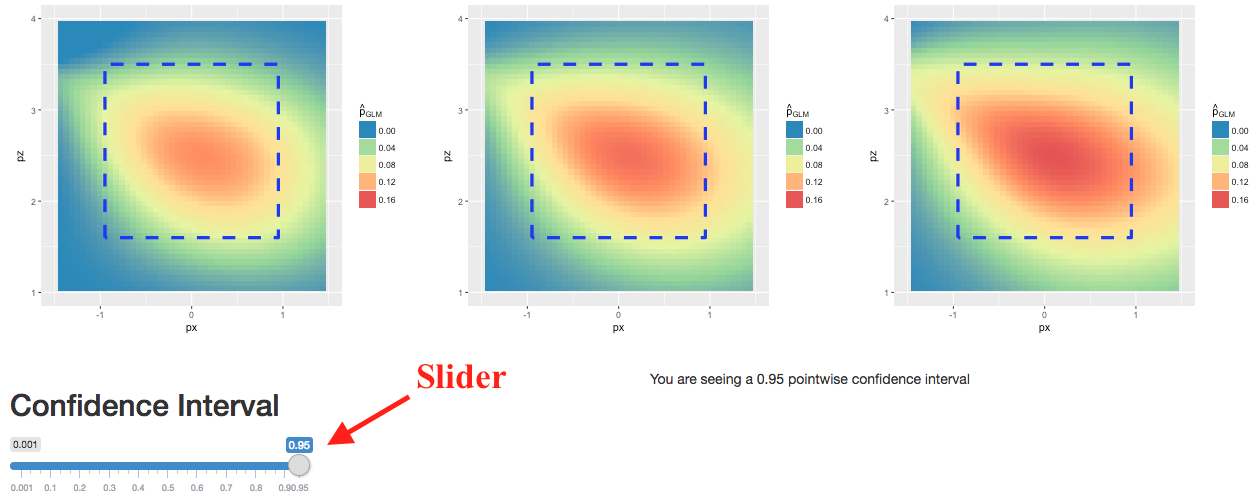
\includegraphics[scale=.32]{Images/95.png}
	\caption{A static image of an interactive heat map confidence interval implemented with Shiny. The user adjusts the slider in the lower left to move {\it through} confidence surfaces, controlled by confidence levels. As the user adjusts the slider, the heat map bounds on the left and right give the appropriate layer or confidence surface.}
	\label{fig:Shiny}
	\end{figure}
The slider specifies a confidence interval level. As the user lowers the confidence interval slider setting, the lower bound on the left and the upper bound on the right will ``move'' toward the point estimate, and look increasingly similar to the point estimate heat map in the middle. As the user increases the confidence interval, the bounds ``move'' away from the point estimate: the lower bound colors cool, while the upper bound colors warm.

In Figure \ref{fig:sequence} we show a sequence of static images in which the slider progressively narrows the confidence interval.
  \begin{figure}[H]
	\centering
	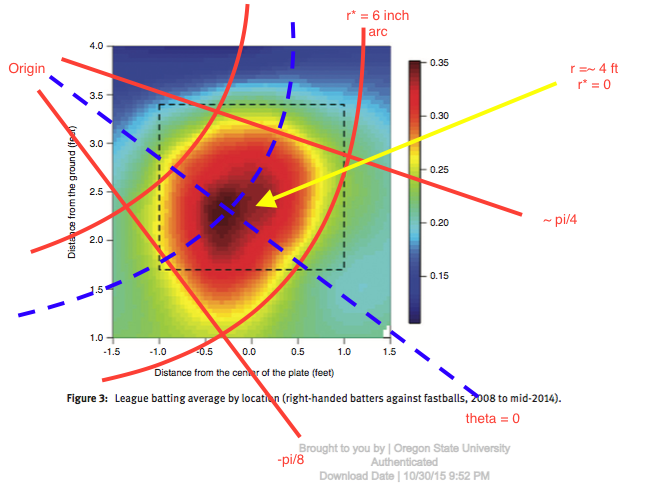
\includegraphics[scale=.25]{Images/1.png}
	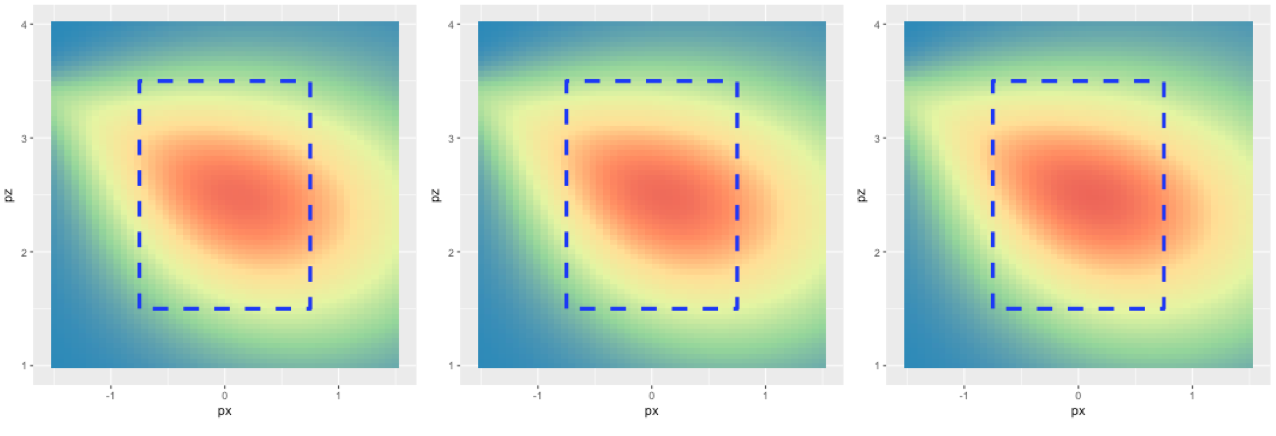
\includegraphics[scale=.25]{Images/25.png}
	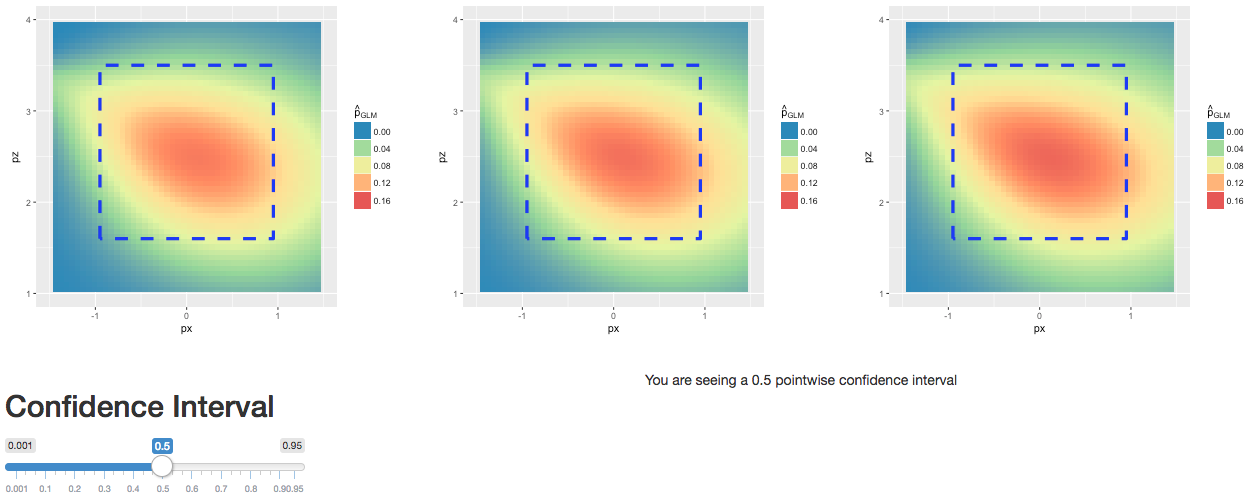
\includegraphics[scale=.25]{Images/50.png}
	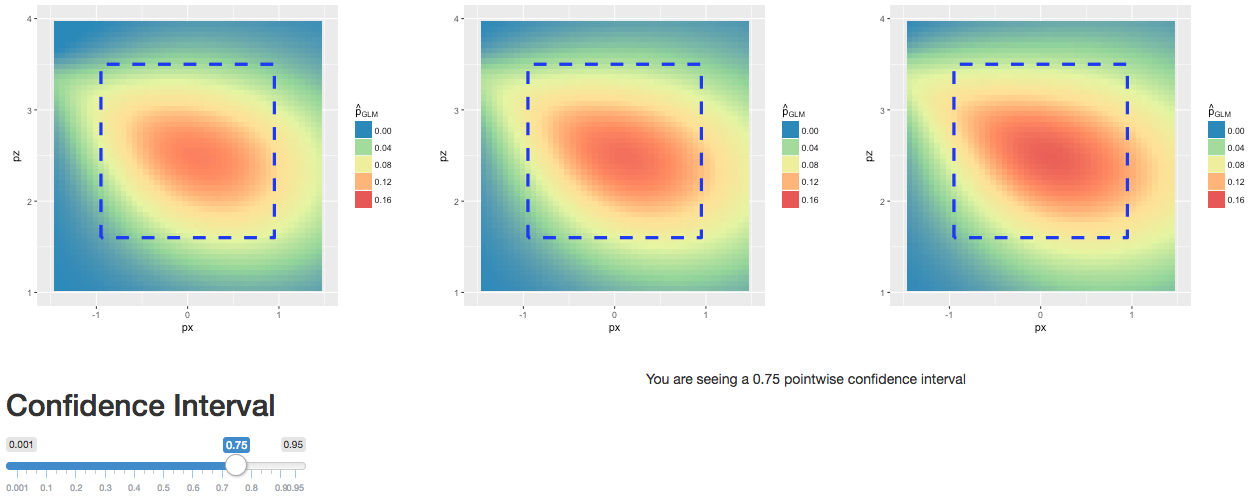
\includegraphics[scale=.25]{Images/75.png}
	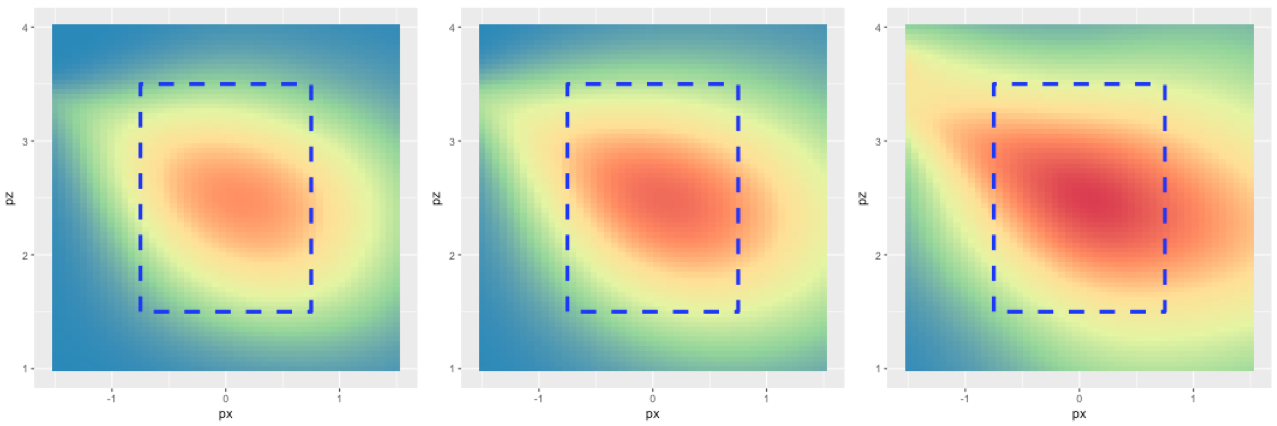
\includegraphics[scale=.25]{Images/99.png}
	\caption{An interactive confidence interval in Shiny lets the user move ``through'' the interval \citep{Shiny}. As the user adjusts the slider in the lower left (shown with first set of three maps), the heat map bounds respond accordingly. In the middle column the point estimate map remains fixed. The lower (column one) and upper (column three) bounds get wider moving from top row to bottom row: 1\%, 25\%, 50\%, 75\%, 99\%.}
	\label{fig:sequence}
	\end{figure}
In Figure \ref{fig:sequence} we show the slider for the first row only. The unchanging middle column contains the point estimate map. The top row shows a 1\% confidence interval, followed by 25\%, 50\%, 75\%, and 99\% in the following rows; the first column contains all lower bounds, the third column all upper bounds. The first row contains three virtually identical maps, with the point estimate in the middle. Moving down the third (upper bound) column of maps, notice how the angled red oval shape subtly grows and elongates. This slow morphing culminates in the final image, where the red oval bleeds out of the strike zone to the upper left, and off the map to right. On the other hand, moving down the first (lower bound) column notice the red oval shrinking. The live, interactive application animates these effects, conveying them more vividly.

\subsection{Discussion}

While the paper version resembles the customary presentation, the actual interactive confidence interval application comes to life as the user adjusts the slider. The user watches the confidence interval bound maps morph into the point estimate map, which fills the intuitive gap explained above. Whereas our mind easily fills in a customary two-dimensional confidence interval on the number line, the Shiny application now fills in the two-dimensional color surfaces of a heat map confidence interval.

To provide wider access to our interactive confidence intervals, we created a R package called {\bf mapapp} that automates creating interactive heat map confidence intervals. The vignette in the next section introduces users to {\bf mapapp}, and guides them through some of its features. 

\section{ An R Package: {\bf mapapp}}

\section{Conclusion}

In this chapter we accomplished three primary objectives. First, we developed a GLM to help explain spatial variation in success probability for baseball hitters. We used biomechanical principles and polar coordinates to create covariates related to pitch location. Second, we developed a new, interactive tool for presenting heat map confidence intervals. We implemented the method in RStudio's Shiny, a web application development framwork. Third, we introduced our newly launched package {\bf mapapp}, designed to help users create their own interactive heat map confidence intervals in Shiny. The last section consists of a {\bf mapapp} instructional vignette.

In the next chapter we augment the GLM with a spatial random effect, and explore approaches for dealing with the vastly increased computational burden.

